\documentclass[tog]{acmsiggraph}

\usepackage{mystyle}

\usepackage{MyMnSymbol} % fixes underbrace command
\usepackage{xcolor}
\usepackage{microtype}
\usepackage{pbox}

\TOGonlineid{0000}
\TOGvolume{0}
\TOGnumber{0}
\TOGarticleDOI{1111111.2222222}
% \TOGprojectURL{}
% \TOGvideoURL{}
% \TOGdataURL{}
% \TOGcodeURL{}

%

\title{{\small Supplemental material for:}\\Entropic Metric Alignment for Correspondence Problems}

\author{}
\pdfauthor{}
\keywords{}

\begin{document}

\teaser{
\fbox{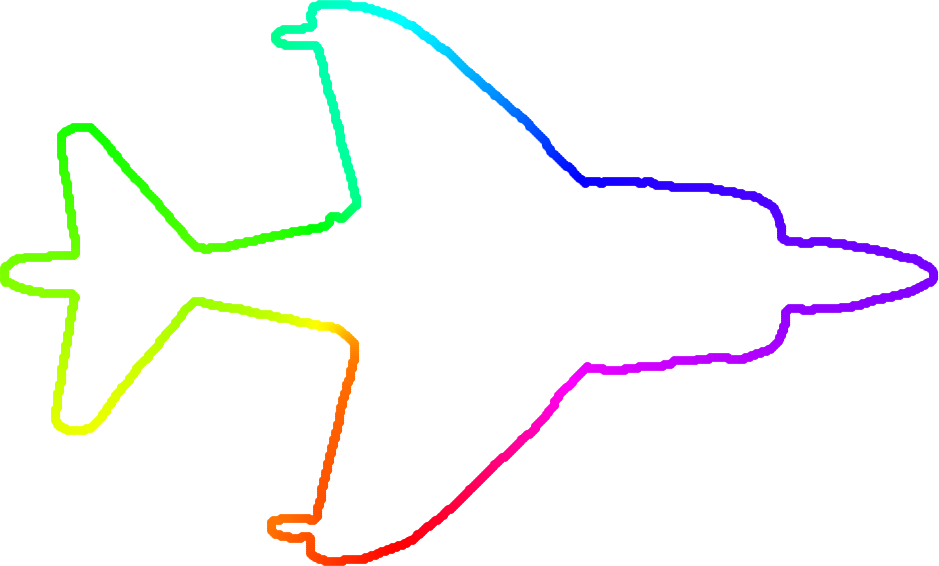
\includegraphics[scale=.1]{figures/2d_shape_match/source.pdf}}\ \ \foreach \n in {1,...,19}{\includegraphics[scale=.1]{figures/2d_shape_match/target\n.pdf}\ \ }\\
\fbox{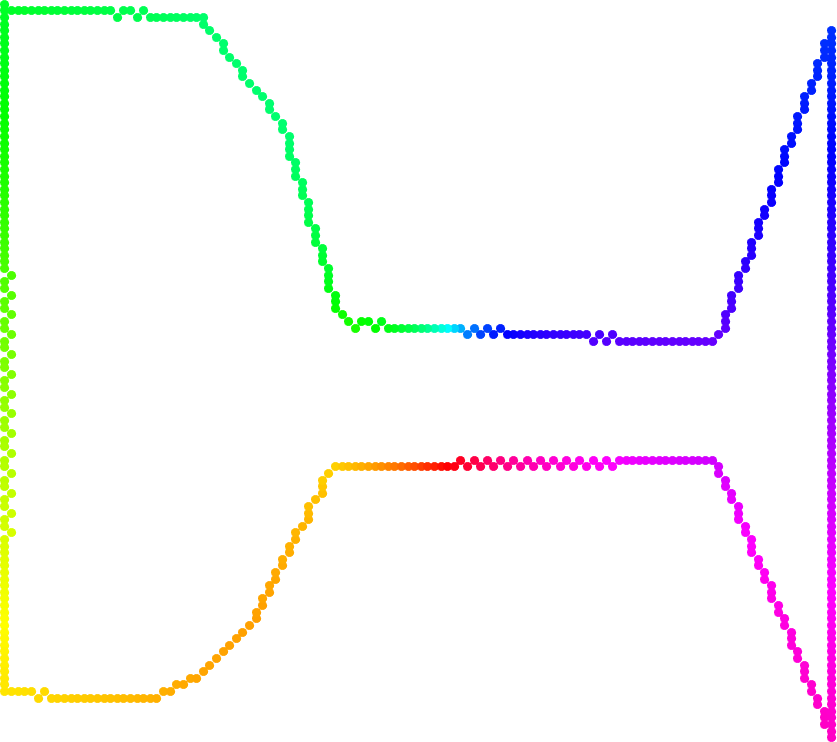
\includegraphics[scale=.1]{figures/2d_shape_match/source_glass.pdf}}\ \ \foreach \n in {1,...,19}{\includegraphics[scale=.1]{figures/2d_shape_match/target_glass\n.pdf}\ \ }\\
\fbox{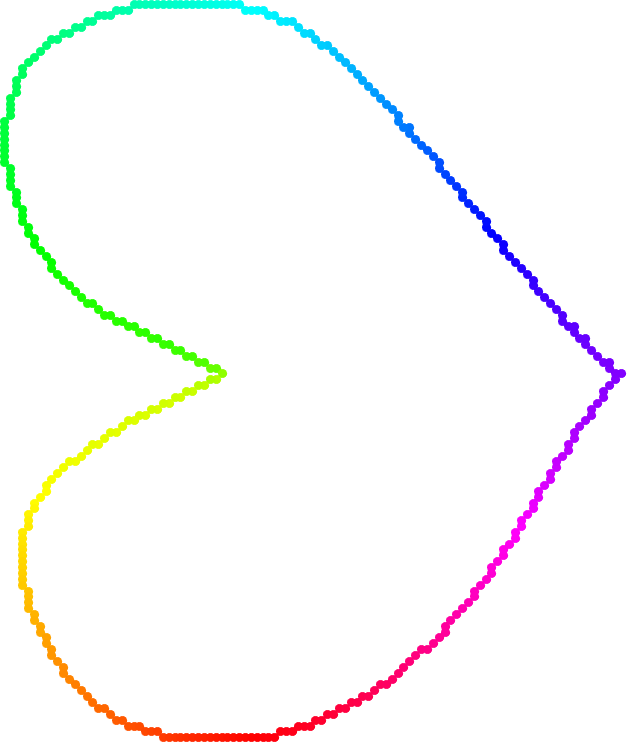
\includegraphics[scale=.1]{figures/2d_shape_match/source_heart.pdf}}\ \ \foreach \n in {1,...,19}{\includegraphics[scale=.1]{figures/2d_shape_match/target_heart\n.pdf}\ \ }\\
\fbox{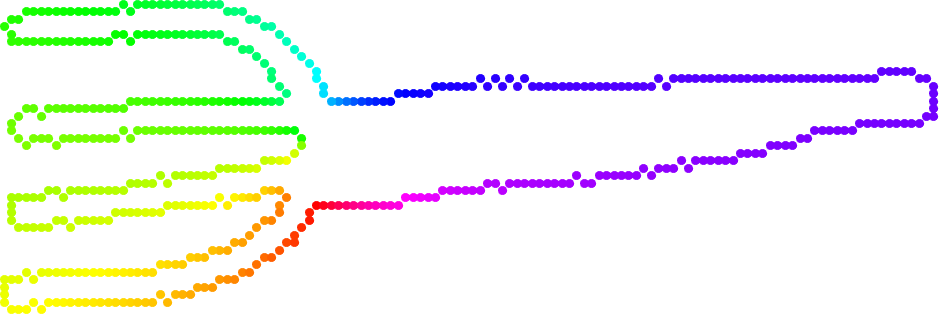
\includegraphics[scale=.1]{figures/2d_shape_match/source_fork.pdf}}\ \ \foreach \n in {1,...,19}{\includegraphics[scale=.1]{figures/2d_shape_match/target_fork\n.pdf}\ \ }
\caption{2D shape matching; color on the boxed model is transferred to the remaining models ($\alpha\equiv7.5\times10^{-4}$).}\label{fig:2d_shape}
\ \\\ \\\vspace{-.1in}
\begin{tabular}{c@{\,}c@{}c@{}c@{}c@{}c@{}c@{}c@{}}
\rotatebox{90}{\small \ \ \ \ \ \ \ \ \ Source}&\foreach \n in {1,...,6}{\includegraphics[width=.15\linewidth]{figures/fro/source\n.pdf}\ \ }\\
\rotatebox{90}{\small \ \ [Aflalo et al.]}&\foreach \n in {1,...,6}{\includegraphics[width=.15\linewidth]{figures/fro/fro\n.pdf}\ \ }\\
\rotatebox{90}{\small \ \ \ \ \ \ Ours}&\foreach \n in {1,...,6}{\includegraphics[width=.15\linewidth]{figures/fro/gw\n.pdf}\ \ }\\
\end{tabular}
\vspace{-.1in}
\caption{Comparison to~\protect\cite{aflalo-2015}.  Here, we compute a map between 2D airplane shapes (data from~\protect\cite{thakoor-2007}), using Euclidean distances in $\D_0$ and $\D$.  The first row shows points marked on the source shape, and the second row shows their mapped targets using their method (top) and ours (bottom).  \GWa successfully recovers a near-bijective map, while~\protect\cite{aflalo-2015} superposes some but not all symmetries (compare columns 2 and 5).}\label{fig:kimmel}
}

\maketitle

%\begin{figure*}\centering
%\end{figure*}


\bibliographystyle{acmsiggraph}
\bibliography{gw}

\end{document}
